% Class 3 — Literature → Protocol
% Overleaf: upload this folder, set compiler to pdfLaTeX, open main.tex
\documentclass[
  english,
  aspectratio=169,
]{beamer}

\usepackage{babel}
\usepackage[utf8]{inputenc}
\usepackage[T1]{fontenc}
\usepackage{booktabs}
\usepackage{tabularx}
\usepackage{multirow}
\usepackage{hyperref}
\usepackage{tikz}

\mode<beamer>{
  \definecolor{links}{HTML}{2A1B81}
  \hypersetup{colorlinks, linkcolor=, urlcolor=links}
  \usetheme{AGH}
}

% Fix title page overlap with AGH header text (16:9 needs more top offset)
\makeatletter
\setbeamertemplate{title page}{%
  \vspace*{2.6cm}%
  \vbox{}%
  \vfill
  \hspace*{0.01\paperwidth}%
  \begingroup
  \centering
  \begin{beamercolorbox}[rounded=true,shadow=true,sep=8pt,wd=0.6\textwidth,center]{title}
    \usebeamerfont{title}\inserttitle\par
    \ifx\insertsubtitle\@empty\else
      \vskip0.25em
      {\usebeamerfont{subtitle}\usebeamercolor[fg]{subtitle}\insertsubtitle\par}%
    \fi
  \end{beamercolorbox}
  \vskip1em\par
  \begin{beamercolorbox}[sep=8pt,center]{author}
    \usebeamerfont{author}\insertauthor
  \end{beamercolorbox}
  \begin{beamercolorbox}[sep=8pt,center]{institute}
    \usebeamerfont{institute}\insertinstitute
  \end{beamercolorbox}
  \begin{beamercolorbox}[sep=8pt,center]{date}
    \usebeamerfont{date}\insertdate
  \end{beamercolorbox}
  \endgroup
  \vfill
}
\makeatother

\title[When Do GNNs Help?]{When Do Graph Neural Networks Help?}
\subtitle{Class 3 --- Literature \& Experimental Protocol}
\author[M.~Bro\'{s} \& M.~Burda]{%
  Micha\l{} Bro\'{s}\inst{1}
  \and
  Micha\l{} Burda\inst{1}
}
\institute[AGH]{%
  \inst{1}%
  Computational Intelligence \\
  Prof.~Adrian Horzyk \\
  AGH University of Krakow
}
\date{} % Class 3 already in subtitle; empty date avoids low duplicate text

\begin{document}

%---------------------------------------------------------------------
\begin{frame}[plain]
  \titlepage
\end{frame}

%#####################################################################
\section{Project reminder}
%#####################################################################

\begin{frame}{01~~What we are building}
  \textbf{Goal:} answer one research question with a fair experiment ---
  not ``train as many models as possible''.

  \vspace{0.6em}
  \begin{block}{Project in one sentence}
    When do graph connections help node classification,
    and when are simple tabular models (MLP / XGBoost) enough?
  \end{block}

  \begin{itemize}
    \item \textbf{Task:} predict a node's class (e.g.\ paper topic)
    \item \textbf{Tabular models:} use node features only (ignore edges)
    \item \textbf{GNNs:} also use neighbours via edges
    \item \textbf{Stress tests:} remove real edges / add fake edges
  \end{itemize}
\end{frame}

\begin{frame}{02~~Research question and hypotheses}
  \begin{block}{Research question}
    When do GNNs beat MLP / XGBoost, and how much edge noise
    can they survive before losing?
  \end{block}

  \begin{enumerate}
    \item \textbf{H1 (breaking point):}
      on clean similar graphs GNNs win;
      after adding $\sim$30\% random fake edges, MLP / XGBoost become better.
    \item \textbf{H2 (similar vs mixed):}
      on mixed / heterophilous graphs, tabular models beat basic GNNs
      from the start.
  \end{enumerate}
\end{frame}

%#####################################################################
\section{Literature}
%#####################################################################

\begin{frame}{03~~Literature overview}
  \textbf{Requirement:} $\geq$3 papers / person, $\geq$6 unique papers in a pair.

  \vspace{0.5em}
  \begin{itemize}
    \item Anchor paper (Platonov et al., ICLR 2023) assigned to \textbf{M.~Burda}
    \item Each student can explain claim, evidence, limitation, project use
    \item Full reading matrix: \texttt{LITERATURE.csv}
  \end{itemize}

  \vspace{0.6em}
  \begin{columns}[T]
    \begin{column}{0.48\textwidth}
      \textbf{Micha\l{} Bro\'{s}}
      \begin{itemize}
        \item Huang et al.\ --- C\&S (ICLR'21)
        \item Kipf \& Welling --- GCN (ICLR'17)
        \item Veli\v{c}kovi\'{c} et al.\ --- GAT (ICLR'18)
      \end{itemize}
    \end{column}
    \begin{column}{0.48\textwidth}
      \textbf{Micha\l{} Burda}
      \begin{itemize}
        \item Platonov et al.\ --- heterophily (ICLR'23)
        \item Hamilton et al.\ --- GraphSAGE (NeurIPS'17)
        \item Zhu et al.\ --- beyond homophily (NeurIPS'20)
      \end{itemize}
    \end{column}
  \end{columns}
\end{frame}

\begin{frame}{04~~Anchor paper}
  \begin{block}{Platonov et al.\ (ICLR 2023)}
    \emph{A Critical Look at the Evaluation of GNNs under Heterophily}
  \end{block}

  \begin{itemize}
    \item \textbf{Claim:} popular heterophily benchmarks can be flawed
      (e.g.\ duplicates in Chameleon / Squirrel $\rightarrow$ leakage);
      on cleaner mixed graphs, strong simple models / standard GNNs
      often beat specialised heterophily GNNs.
    \item \textbf{Evidence:} duplicate analysis; new / revised datasets
      (incl.\ Roman-empire); MLP / GBDT-style vs GNN comparisons.
    \item \textbf{Limitation:} not a controlled edge-noise protocol.
    \item \textbf{Our use:} similar vs mixed setup; dataset choice;
      justification that tabular models can win.
  \end{itemize}
\end{frame}

\begin{frame}{05~~Reading matrix (summary)}
  \begin{block}{Assigned papers}
    \scriptsize
    \renewcommand{\arraystretch}{1.2}
    \begin{tabular}{p{2.2cm}p{4.2cm}p{4.4cm}}
      \textbf{Reader} & \textbf{Paper} & \textbf{Project use} \\
      \hline
      M.~Burda & Platonov ICLR'23 & Anchor; homo/hetero; datasets \\
      M.~Bros & Huang C+S ICLR'21 & Strong non-GNN comparator \\
      M.~Bros & Kipf GCN ICLR'17 & Main GNN (Exp.\ A) \\
      M.~Bros & GAT ICLR'18 & Attention GNN comparator \\
      M.~Burda & GraphSAGE NeurIPS'17 & Main GNN (Exp.\ B) \\
      M.~Burda & Zhu NeurIPS'20 & Why GNNs fail under heterophily \\
    \end{tabular}
  \end{block}

  \vspace{0.4em}
  {\small Full columns in CSV: claim and evidence, limitation, project use.}
\end{frame}

%#####################################################################
\section{Experimental protocol}
%#####################################################################

\begin{frame}{06~~Datasets and splits}
  \begin{columns}[T]
    \begin{column}{0.55\textwidth}
      \begin{block}{4 public graphs (PyG)}
        \scriptsize
        \renewcommand{\arraystretch}{1.15}
        \begin{tabular}{llcc}
          Dataset & Nodes & Same-class & Type \\
          \hline
          Cora & 2.7k & 81\% & Similar \\
          PubMed & 19.7k & 80\% & Similar \\
          Chameleon* & 2.3k & 23\% & Mixed \\
          Roman-empire & 22.7k & 5\% & Mixed \\
        \end{tabular}
        \vspace{0.35em}

        {\scriptsize * Prefer filtered Chameleon (Platonov) -- no duplicates.}
      \end{block}
    \end{column}
    \begin{column}{0.42\textwidth}
      \begin{block}{Splits}
        Fixed train / val / test \\
        Same splits for all models \\
        Preprocessing fit on train only
      \end{block}
      \begin{block}{Resources}
        Laptop / Colab \\
        $\sim$2--10\,s per run \\
        under 50\,MB data
      \end{block}
    \end{column}
  \end{columns}
\end{frame}

\begin{frame}{07~~Models we compare}
  \begin{columns}[T]
    \begin{column}{0.48\textwidth}
      \begin{block}{No graph (0\% edges)}
        \begin{itemize}
          \item MLP (features only)
          \item XGBoost / LightGBM
          \item Optional: MLP + Correct\&Smooth
        \end{itemize}
      \end{block}
    \end{column}
    \begin{column}{0.48\textwidth}
      \begin{block}{With graph}
        \begin{itemize}
          \item GCN --- averages neighbours
          \item GAT --- learns edge weights
          \item GraphSAGE --- samples neighbours
        \end{itemize}
      \end{block}
    \end{column}
  \end{columns}

  \vspace{0.8em}
  \textbf{Start scope (MVP):}
  Cora + one mixed dataset;
  MLP, XGBoost, GCN, GraphSAGE.
  GAT and C\&S as extensions.
\end{frame}

\begin{frame}{08~~Metrics and fair protocol}
  \begin{itemize}
    \item \textbf{Primary metric:} accuracy (node classification)
    \item \textbf{Secondary:} macro-F1 (if class imbalance)
    \item \textbf{Seeds:} 5 random seeds; report mean $\pm$ spread
    \item \textbf{Fair tuning:} same train/val/test; comparable HP budget
    \item \textbf{Logging:} settings, seeds, raw metrics, runtime / hardware
  \end{itemize}

  \vspace{0.6em}
  \begin{alertblock}{What would change our mind?}
    If GNNs stay ahead under high fake-edge noise on similar graphs,
    or beat tabular models on mixed graphs -- H1 / H2 are weakened.
  \end{alertblock}
\end{frame}

\begin{frame}{09~~Experiment A -- deleting edges}
  \textbf{Idea:} randomly remove true edges: 0\%, 20\%, 40\%, 60\%, 80\%, 100\%.

  \vspace{0.5em}
  \begin{itemize}
    \item At 100\% the GNN has no neighbours $\approx$ feature-only model
    \item Question: how much real structure is needed for GNNs to win?
  \end{itemize}

  \vspace{0.4em}
  \begin{center}
  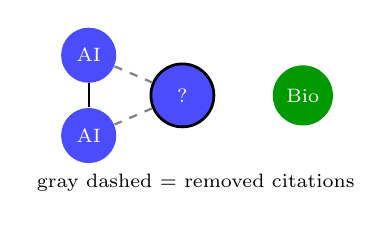
\begin{tikzpicture}[scale=0.85, every node/.style={font=\scriptsize}]
    \node[circle, fill=blue!70, text=white, minimum size=0.7cm] (a1) at (0,1.2) {AI};
    \node[circle, fill=blue!70, text=white, minimum size=0.8cm, draw=black, line width=1pt] (q) at (1.4,0.6) {?};
    \node[circle, fill=blue!70, text=white, minimum size=0.7cm] (a2) at (0,0) {AI};
    \node[circle, fill=green!60!black, text=white, minimum size=0.7cm] (b1) at (3.2,0.6) {Bio};
    \draw[gray, dashed, thick] (a1) -- (q);
    \draw[gray, dashed, thick] (q) -- (a2);
    \draw[black, thick] (a1) -- (a2);
    \node at (1.6,-0.7) {gray dashed = removed citations};
  \end{tikzpicture}
  \end{center}
\end{frame}

\begin{frame}{10~~Experiment B -- fake edges}
  \textbf{Idea:} keep true edges; add random wrong edges $0\% \rightarrow 75\%$.

  \vspace{0.5em}
  \begin{itemize}
    \item AI paper gets linked to a random Bio paper
    \item Hypothesis: after $\sim$30\% noise, tabular models overtake GNNs
    \item Tabular baselines stay flat (they ignore edges)
  \end{itemize}

  \vspace{0.3em}
  \begin{center}
  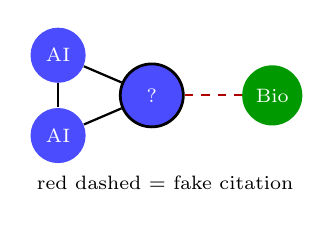
\begin{tikzpicture}[scale=0.85, every node/.style={font=\scriptsize}]
    \node[circle, fill=blue!70, text=white, minimum size=0.7cm] (a1) at (0,1.2) {AI};
    \node[circle, fill=blue!70, text=white, minimum size=0.8cm, draw=black, line width=1pt] (q) at (1.4,0.6) {?};
    \node[circle, fill=blue!70, text=white, minimum size=0.7cm] (a2) at (0,0) {AI};
    \node[circle, fill=green!60!black, text=white, minimum size=0.7cm] (b1) at (3.2,0.6) {Bio};
    \draw[black, thick] (a1) -- (q);
    \draw[black, thick] (q) -- (a2);
    \draw[black, thick] (a1) -- (a2);
    \draw[red!70!black, dashed, thick] (q) -- (b1);
    \node at (1.6,-0.7) {red dashed = fake citation};
  \end{tikzpicture}
  \end{center}
\end{frame}

\end{document}
